\section{Security Model}
\label{sec:attestation}

The rest of this section describes the security properties of
enclaves, discussing the trade-offs made while trying to balance security with
backwards compatibility.

Enclaves were designed to contain and protect the privacy-sensitive parts of an
application. All the code that handles private data must receive integrity
protection. Otherwise, a hostile environment could modify the code to leak
information about private data. Therefore, the SGX programming model prescribes
that code which accesses private data must be entirely contained inside an
enclave. Jumping into and out of enclave code must be performed explicitly
using the dedicated instructions \texttt{EENTER} and \texttt{EEXIT}.

\begin{figure}[hbtp]
  \center{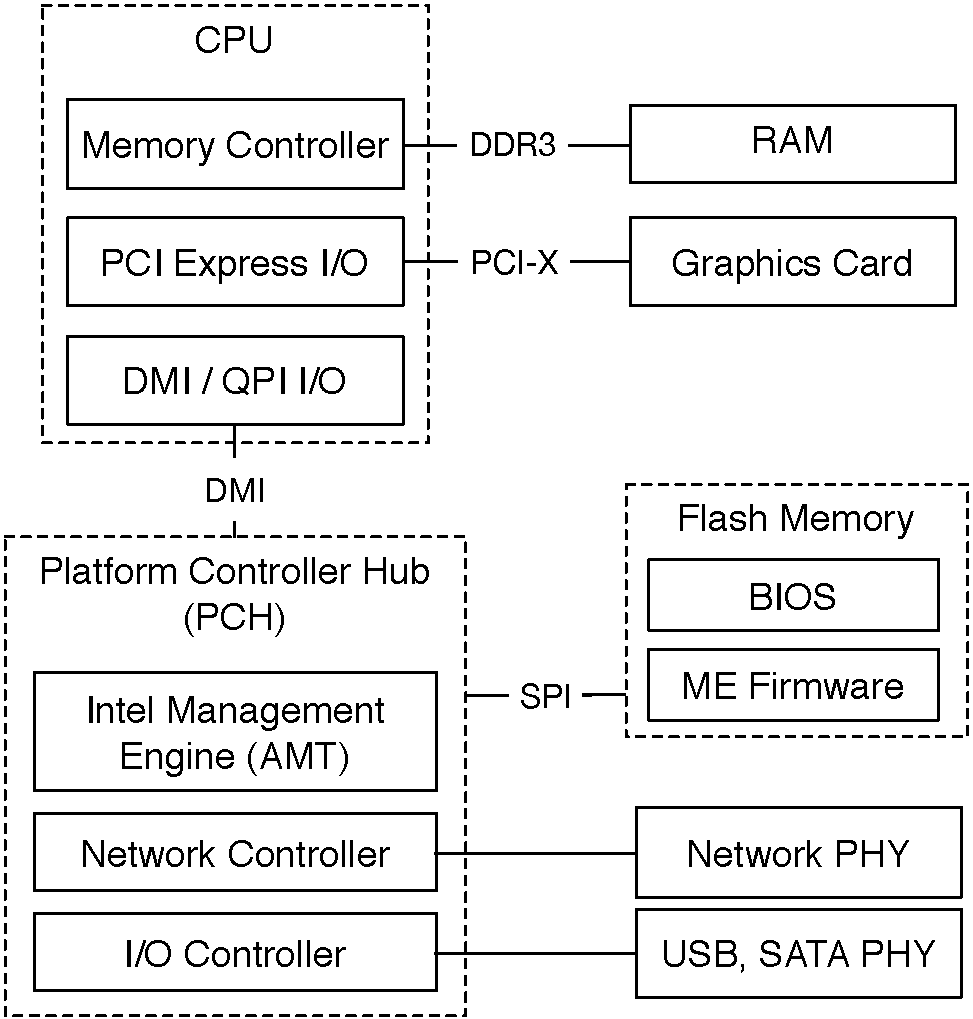
\includegraphics[width=65mm]{figures/pch.pdf}}
  \caption{
    The architecture of modern Intel systems.
    The Platform Controller Hub (PCH) contains a service processor, called the
    Intel Management Engine (ME). The processor has direct access to the
    network, can read and modify RAM via DMA transfers, and can override the
    CPU boot vector. The processor runs firmware stored in the same flash
    memory as the BIOS code.
  }
  \label{fig:pch}
\end{figure}


